%%%%%%%%%%%%%%%%%%%%%%%%%%%%%%%%%%%%%%%%%
% University Assignment Title Page 
% LaTeX Template
% Version 1.0 (27/12/12)
%
% This template has been downloaded from:
% http://www.LaTeXTemplates.com
%
% Original author:
% WikiBooks (http://en.wikibooks.org/wiki/LaTeX/Title_Creation)
%
% License:
% CC BY-NC-SA 3.0 (http://creativecommons.org/licenses/by-nc-sa/3.0/)
% 
% Instructions for using this template:
% This title page is capable of being compiled as is. This is not useful for 
% including it in another document. To do this, you have two options: 
%
% 1) Copy/paste everything between \begin{document} and \end{document} 
% starting at \begin{titlepage} and paste this into another LaTeX file where you 
% want your title page.
% OR
% 2) Remove everything outside the \begin{titlepage} and \end{titlepage} and 
% move this file to the same directory as the LaTeX file you wish to add it to. 
% Then add \input{./title_page_1.tex} to your LaTeX file where you want your
% title page.
%
%%%%%%%%%%%%%%%%%%%%%%%%%%%%%%%%%%%%%%%%%
%\title{Title page with logo}
%----------------------------------------------------------------------------------------
%	PACKAGES AND OTHER DOCUMENT CONFIGURATIONS
%----------------------------------------------------------------------------------------

\documentclass[12pt, a4paper]{report}
\usepackage{hyperref}
\usepackage[english]{babel}
\usepackage[utf8]{inputenc}
\usepackage{amsmath}
\usepackage{amsfonts}
\usepackage{graphicx}
\usepackage[version=4]{mhchem}
\graphicspath{{Figures/}}
\setcounter{secnumdepth}{2} % set dept of numeration in section (1.1.1)
\setcounter{tocdepth}{2} % set dept of section to show in table of contents
\usepackage{indentfirst}
\usepackage{url}
\usepackage{listings}
\usepackage{tabu}
\usepackage{subfiles}
\usepackage{blindtext}
\usepackage{float}
\usepackage{dirtree}
\usepackage[left=3cm,right=3cm,top=3cm]{geometry} % set the margin
\usepackage{changepage}
\usepackage{fancyhdr}
\usepackage{dirtytalk}
\usepackage{caption}
\usepackage{subcaption}
\usepackage{booktabs}
\usepackage{longtable}
\usepackage[absolute,overlay]{textpos}
\captionsetup[figure]{labelfont=it,textfont={it}}
% \usepackage{enumitem}
\usepackage[inline]{enumitem}
\usepackage{array}
\usepackage{comment}
\usepackage{diagbox}
\usepackage{multirow}
%\renewcommand{\baselinestretch}{1.5} % set interline
\pagestyle{fancy}
\fancyhf{}
%\rhead{\rightmark}
\chead{\leftmark}
\cfoot{\thepage}
\renewcommand{\headrulewidth}{2pt}
\renewcommand{\footrulewidth}{1pt}
\usepackage{color,soul}
\usepackage{algorithm}
\usepackage{algpseudocode}
\usepackage{amssymb}
\usepackage{colortbl}
\usepackage{titlesec}
\usepackage{algorithmicx}
\usepackage{algorithm} % http://ctan.org/pkg/algorithms
\usepackage{amsthm, amssymb}
\newtheorem{prop}{Proposition}
\titleformat
{\chapter} % command
[display] % shape
{\scshape\huge} % format
{Chapter \ \thechapter} % label
{0.5ex} % sep
{
    \rule{\textwidth}{2pt}
    \vspace{-0.5ex}
    \centering
} % before-code
[
\vspace{-0.5ex}%
\rule{\textwidth}{0.7pt}
] % after-code
\setlength{\headheight}{15pt}
\begin{document}

\bibliographystyle{ieeetr}

\begin{titlepage}

\newcommand{\HRule}{\rule{\linewidth}{0.5mm}} % Defines a new command for the horizontal lines, change thickness here

\center % Center everything on the page
 
%----------------------------------------------------------------------------------------
%	HEADING SECTIONS
%----------------------------------------------------------------------------------------

\textbf{\huge Università degli Studi di Salerno}\\[0.6cm] % Name of your university/college
\textsc{\Large Dipartimento di ingegneria dell'Informazione ed Elettrica e Matematica applicata}\\[0.2cm]

\begin{figure}[H]
\centering

\includegraphics[width = 0.6\linewidth]{Figures/logo.png}
\end{figure}
\textsc{\Large Ph.D. Program in Information Engineering}\\[0.4cm] % Major heading such as course name

%----------------------------------------------------------------------------------------
%	TITLE SECTION
%----------------------------------------------------------------------------------------

\HRule \\[0.8cm]
{ \huge \bfseries First year report}\\[0.3cm] % Title of your document
\HRule \\[1.5cm]
 
%----------------------------------------------------------------------------------------
%	AUTHOR SECTION
%----------------------------------------------------------------------------------------

\begin{minipage}{0.4\textwidth}
\begin{flushleft} \large
\emph{Author:} \\
dott. Francesco \textsc{Rosa} \newline
\end{flushleft}
\end{minipage}
~
\begin{minipage}{0.37\textwidth}
\begin{flushright} \large
\emph{Supervisor:}\\
Ch.ma. Mario \textsc{Vento}\newline
\end{flushright}
\end{minipage}\\[1.5cm]

% If you don't want a supervisor, uncomment the two lines below and remove the section above
%\Large \emph{Author:}\\
%John \textsc{Smith}\\[3cm] % Your name

%----------------------------------------------------------------------------------------
%	DATE SECTION
%----------------------------------------------------------------------------------------

{\large XXXVII cycle - Academic year 2021/2022}\\[1cm] % Date, change the \today to a set date if you want to be precise

%----------------------------------------------------------------------------------------
%	LOGO SECTION
%----------------------------------------------------------------------------------------
 % Include a department/university logo - this will require the graphicx package
 
%----------------------------------------------------------------------------------------

\vfill % Fill the rest of the page with whitespace
\end{titlepage}

\clearpage
%\section*{\center Abstract}
%\vspace{5 ex}
\chapter*{Overview}\label{chapter:overview}
\addcontentsline{toc}{chapter}{Overview}

This report represents the final document of the first year of the doctorate carried out by the undersigned. The document conforms to the latest version of the document \hyperlink{https://corsi.unisa.it/ingegneria-dell-informazione/didattica/guida-dello-studente}{\textit{\say{Requirements for the PhD degree}}} approved on 14/12/2020 by the professors' college and available on the university platform in the area reserved for doctoral students. As requested, the document contains a report on the activities carried out by the student during the first year. \par
The document is divided, as suggested, in the aforementioned document, into 4 mandatory chapters, Background \ref{chapter:background}, Research Plan \ref{chapter:research_plan}, Preliminary Results \ref{chapter:preliminary_results}, and Other Activities \ref{chapter:other_activities}.
\newline The first chapter contains the Introduction (Section \ref{sec:intro}) and the State-of-the-Art (Section \ref{sec:sota}) sections. The former introduces to the topic of \textit{Learning from Demonstration}, that is the main topic of this report, pointing out the the importance of the field and the existing knowledge. The latter presents the literature review. This section analyzes from a methodological and application perspective the main approaches by which the problem is solved, highlighting the pros and cons of each method.
\newline The second chapter containes the Research Topic (Section \ref{sec:research_topic}) and the Research Plan (Section \ref{sec:research_activity}) sections. The first presents the gaps that can be extrapolated from the State-of-the-Art, with respect to the context of interest. The second reports the proposed research activity, going on to highlight the connection between the proposal and the gaps presented earlier, the importance of the proposal with respect to the context of interest, and the methodological and experimental procedures that will be followed to track and evaluate progress.
\newline The third chapter contains the Dataset Description (Section \ref{sec:dataset_description}) and the Experiment Results (Section \ref{sec:experiment_results}) sections. The former describes the dataset used during the experiments and the type of data that it contains. While the latter reports the results obtained by running the designed experiments.
\newline The fourth chapter shows all the activities carried out during the year, including courses attended at the university, and other research activities.
% \begin{adjustwidth}{38pt}{38pt}
% \textit{Here I write the abtract.}
% \end{adjustwidth}

\chapter{Background [MAX 25 pag.]}
\section{Introduction}
\label{sec:intro}
Robotic technology is one of the pillars of modern society. Thanks to advances in information, electronic, and
mechanical fields, we can build and program machines to solve various tasks in different scenarios, e.g. industrial,
surgery, space missions etc. \newline In manufacturing, given their ability to reproduce the same movement over time
with an high level of accuracy and precision, robots are massively used to solve repetitive and dangerous activities
such as assembly, welding (Figure \ref{fig:welding}) and material handling    (Figure \ref{fig:material_handling}).
\begin{figure}[htb]
     \centering
     %\begin{subfigure}[b]{0.6\textwidth}
     %    \centering
     %    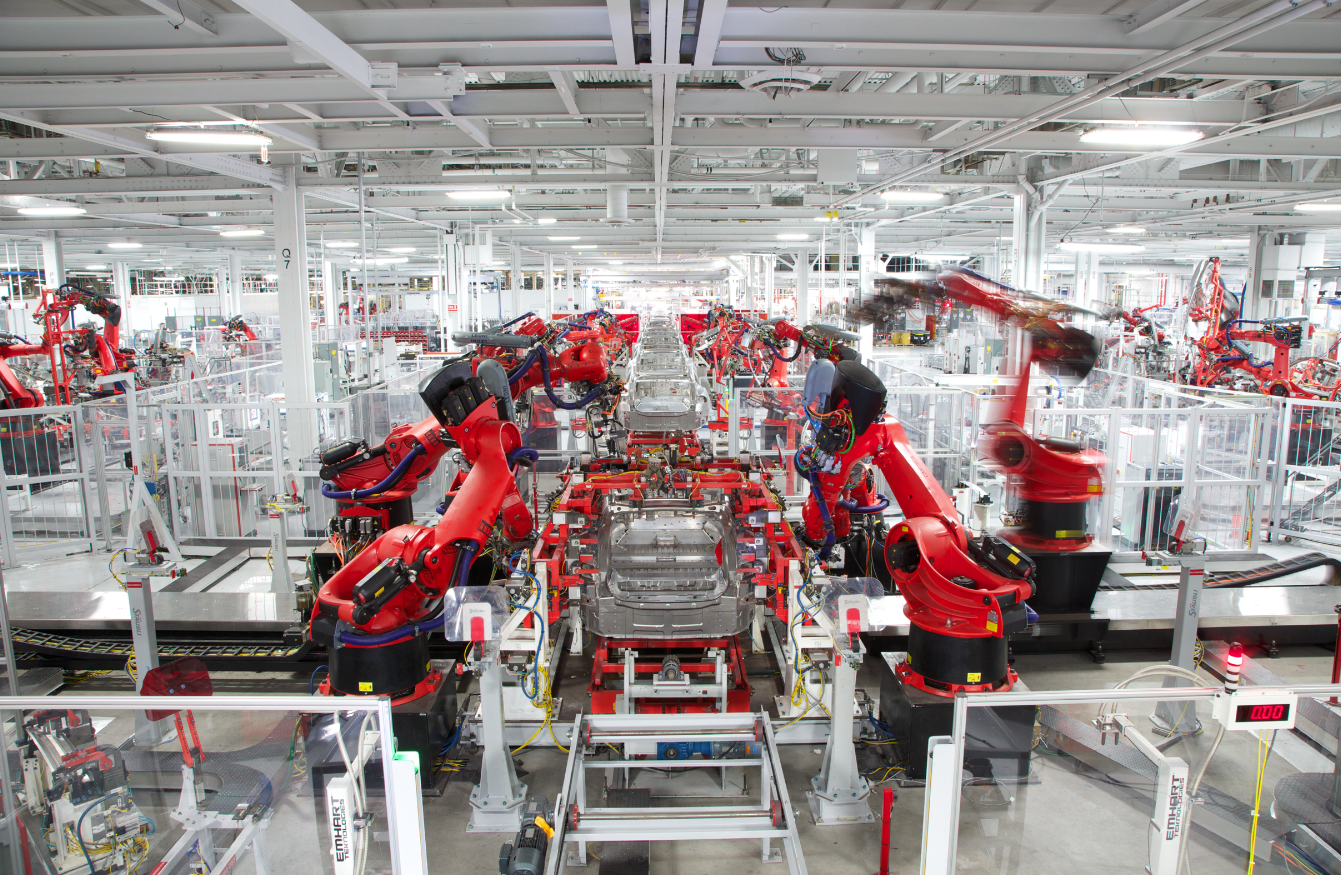
\includegraphics[width=\textwidth]{Figures/images/assembly.jpg}
     %    \caption{Robots involved in Tesla Assembly line}
     %    \label{fig:assembly}
     %\end{subfigure}
     %\hfill
     \begin{subfigure}[b]{0.45\textwidth}
         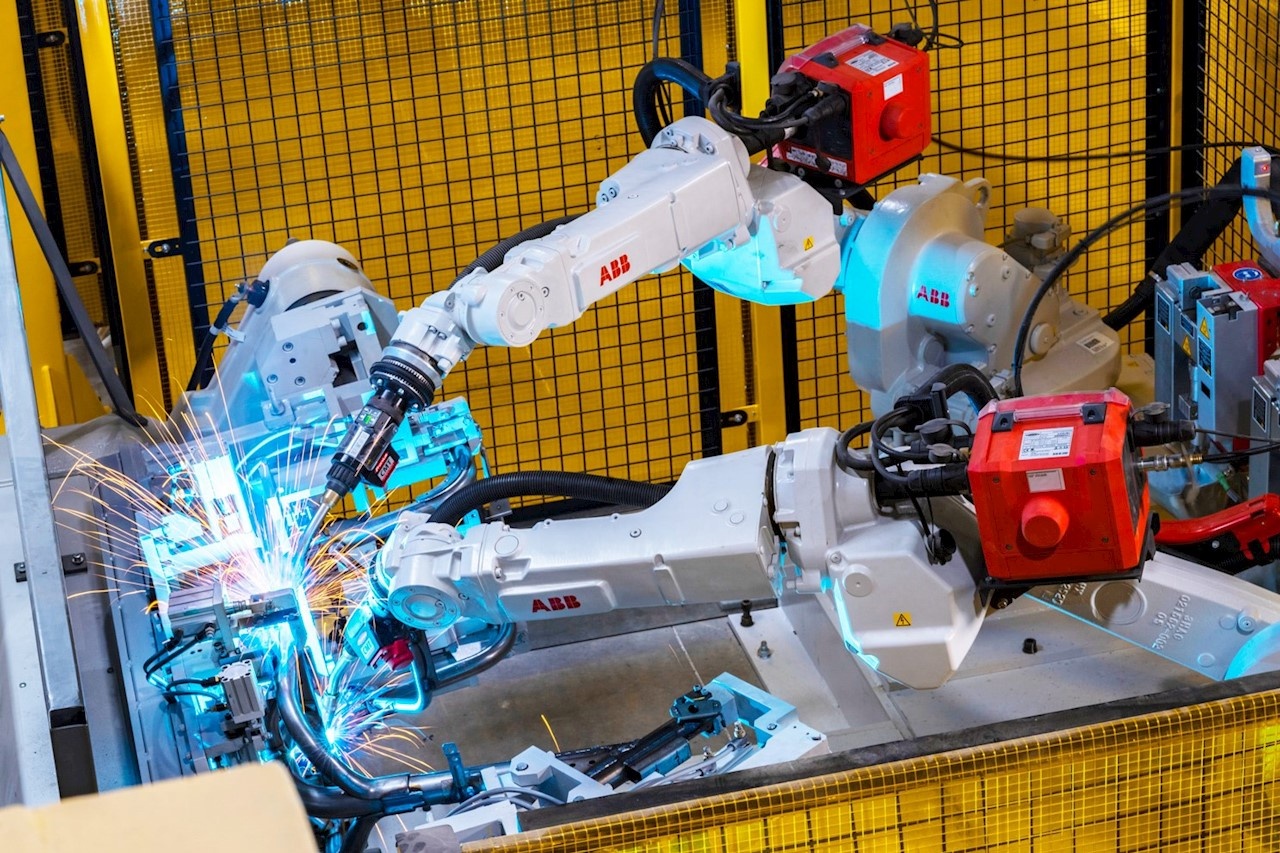
\includegraphics[width=\textwidth]{Figures/images/welding.jpg}
         \caption{Robots involved in arc welding operation}
         \label{fig:welding}
     \end{subfigure}
     \hfill
     \begin{subfigure}[b]{0.5\textwidth}
         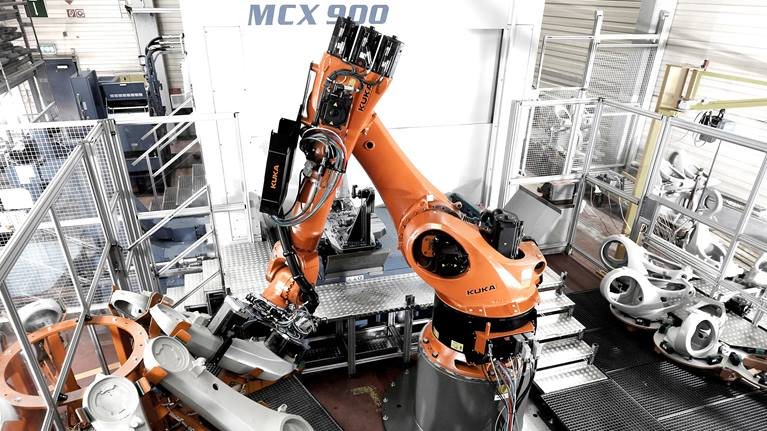
\includegraphics[width=\textwidth]{Figures/images/loading.jpg}
         \caption{Robot involved in loading operation}
         \vspace{0.5cm}
         \label{fig:material_handling}
     \end{subfigure}
    \hfill
    \caption{Industrial Robots: example of applications}
    \label{fig:industrial_robots_example}
\end{figure}


%Given improvements in control techniques and motion precision, robotic systems can reproduce very sensible movements
%needed, for example, in %surgery applications. \medskip \noindent \fcolorbox{red}{yellow}{%
%\minipage[t]{\dimexpr0.48\linewidth-2\fboxsep-2\fboxrule\relax} Inserire immagine Cooperation \endminipage} \medskip
\noindent While in the early day, robotic systems were constrained in isolated and known environments. Over the past few
decades, robots have been asked to solve tasks in dynamic and unknown/partially-known environments, where they must
\textbf{coexist} and \textbf{cooperate} with humans, while  solving different \textbf{dynamic} tasks (e.g. pick a
requested object, whose position is not known a priori). \newline The reason for the increasing demand for such
applications may be found in factors such as:
\begin{enumerate}[label=(\alph*)]
    \item The affirmation of the \textit{Industry 4.0} paradigm, in which the various phases of a factory are linked to
    each other and therefore the robots must be in communication with each other and be able to adapt to changes in the
    production phases.
    \item The spreading of \textit{social robots} (e.g. Pepper \cite{pepper}), that find their appeal in highly
    unstructured applications such as household or shop-recommendation systems.      
    \item The increasing availability of the so-called \textit{cobots} (e.g. Franka Emika Panda robot \cite{panda}),
    which are low-cost robots that allow the automation of light load processes (e.g. drilling, palletizing, polishing)
    while sharing the workspace with humans or other robots. Thanks to cobots, also small factories, that were left out
    from this automation process because of the high-cost of previous solutions, can now start to automate their
    production phases, contributing to increase the demand.
\end{enumerate}
In this scenario, the desired characteristics of such robotic systems are:\begin{enumerate*}[label=\textbf{(\alph*)}]
    \item The capability to exhibit \textit{``intelligent" behaviors} during the task execution in response to dynamic
    changes in the environmental condition (e.g. pre-grasping manipulation \cite{kalashnikov2018qt_opt}, motor failure
    and environmental uncertainties \cite{anne2021meta_learning_fast_adaptive}).
    \item The ability to easily \textit{adapt} to new tasks \cite{jang2022bc_z}. 
\end{enumerate*}
\newline These requirements can be difficult to obtain with typical robotic programming techniques based on hand-written
policy, and control techniques which require a careful analysis of the process dynamics, the building of an analytic
model, and finally, the derivation of a control law that meets certain design criteria
\cite{hafner2011reinforcement_in_feedback_controll}. This design process is tedious, and time consuming, especially when
\textbf{high-level perception systems} (e.g. camera, microphones, motion sensors etc.) are used to infer the state of
the environment (e.g. the unknown position of the desired object to pick with respect to the end-effector) and/or the
intention of the human operator. \newline In contrast, very relevant results have been obtained by leveraging
\textit{Learning Techniques}, which exploit \textbf{agent experience} or \textbf{expert demonstration}. Generally, the
former is referred as \textit{Reinforcement Learning} (RL) \cite{sutton2018reinforcement}, while the latter is referred
as \textit{Imitation Learning} (IL) or \textit{Learning from Demonstration} (LfD)
\cite{argall2009robot_learning_from_demonstration}. Both the approaches aim to obtain an artificial agent, that able to
perform correctly a task or a set of tasks by following a learned policy, however the way how this goal is achieved is
quite different. The main differences between RL and IL are related to presence/absence of a reward function, and the
presence/absence of expert demonstrations. \newline Indeed, in RL formalism \cite{kaelbling1996reinforcement_survey},
the learning procedure is based on a \textit{hand-designed reward function}, i.e. a measure of the quality of the
performed action with respect to the task to be executed (e.g. the distance between the current position and the target
one in a reaching task \cite{}), which drives the agent to produce a sequence of actions which maximize the reward.
While in IL formalism \cite{osa2018algorithmic}, the learning procedure is based on the minimization of a
\textit{loss-function} (e.g. Mean-Squared Error \cite{james2013introduction_to_sl}, Hinge-loss \cite{cortes1995support},
Kullback-Leibler divergence \cite{kullback1951information}), which guides the agent to reproduce/mimic the same actions
of the expert. \newline Regarding the possibility to exploit past experience, in RL literature, three approaches can be
found \cite{levine202rl_tutorial}:
\begin{itemize*}
    \item \textbf{\textit{On-policy}} Reinforcement Learning (Figure \ref{fig:onpolicy}), the trained policy is the same
    policy used to collect data, so, the only used past experience is related to the last policy rollout. These methods
    require a considerable amount of interactions to be trained \cite{}.
    \item \textbf{\textit{Off-policy}} Reinforcement Learning (Figure \ref{fig:offpolicy}), there are two policies, the
    behavior policy used to get experience, and the target policy, the policy to evaluate and improve. The target policy
    can exploit past experience during training. These methods are known to be more data-efficient \cite{}, although
    they still require interaction with the environment. 
    \item \textbf{\textit{Offline}} Reinforcement Learning (Figure \ref{fig:offline}), this setting is similar to the
    classic \textit{supervised learning approach}, where the target policy is trained via a \textit{static dataset} $D$,
    collected by an unknown policy $\pi_{\beta}$.  
\end{itemize*}
\begin{figure}[htbp]
     \centering
     \begin{subfigure}[b]{0.25\textwidth}
         \centering
         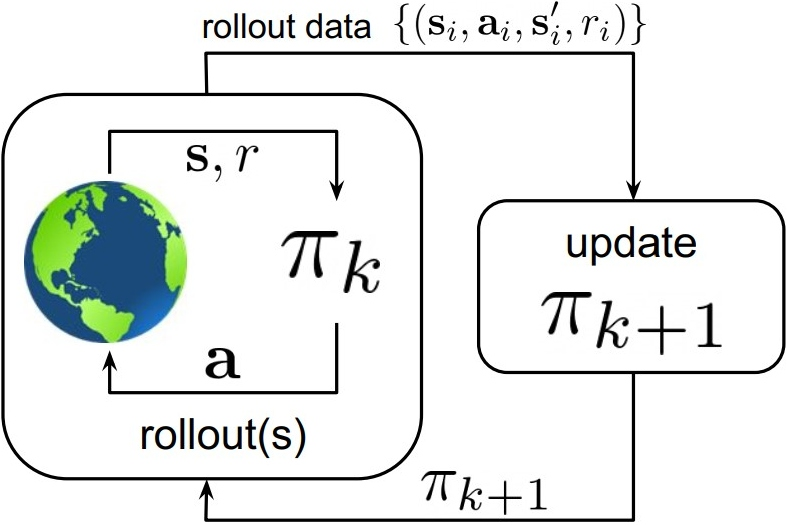
\includegraphics[width=\textwidth]{Figures/images/RL_methods/onpolicy.jpg}
         \caption{On-policy RL}
         \label{fig:onpolicy}
     \end{subfigure}
     \hfill
     \begin{subfigure}[b]{0.25\textwidth}
         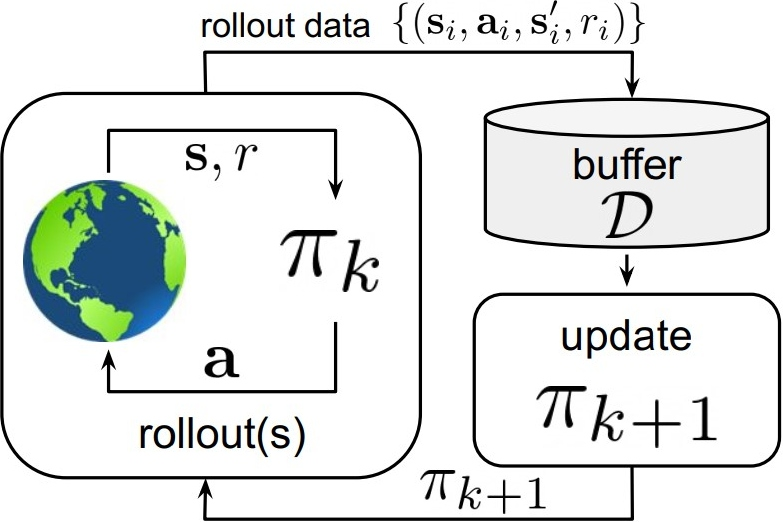
\includegraphics[width=\textwidth]{Figures/images/RL_methods/offpolicy.jpg}
         \caption{Off-policy RL}
         \label{fig:offpolicy}
     \end{subfigure}
     \hfill
     \begin{subfigure}[b]{0.35\textwidth}
         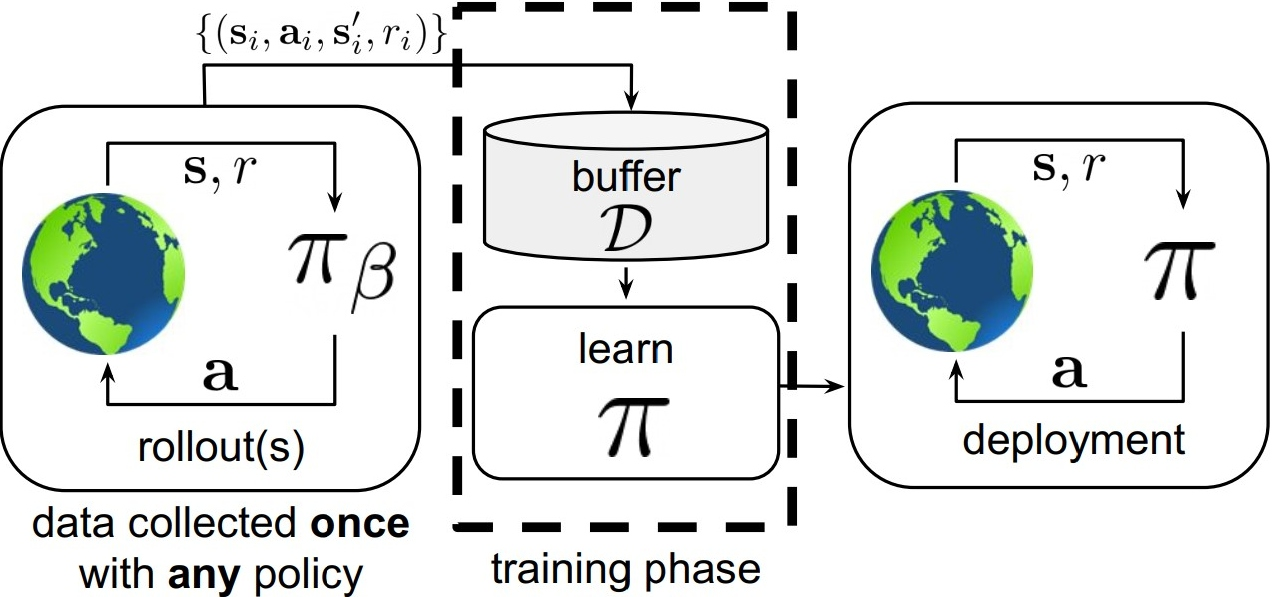
\includegraphics[width=\textwidth]{Figures/images/RL_methods/offline.jpg}
         \caption{Offline RL}
         \label{fig:offline}
     \end{subfigure}
    \hfill
    \caption{Graphical Representation of Reinforcement Learning Methods \cite{levine202rl_tutorial}}
    \label{fig:rl_methods}
\end{figure}


\noindent The need for a task-specific reward function, and the need for expensive and time-consuming training
procedures, are the main difficulties in applying such methods for real-world application
\cite{hussein2017imitation_learning_survey}. \newline As opposed to RL, in IL, the starting point for all the methods
(Figure \ref{fig:il_methods}), is a dataset $D$ containing expert demonstrations (e.g. trajectories of teleoperated
robot \cite{}, video of human pouring a liquid \cite{}). Based on the approach, the information contained in the dataset
is used in different way:
\begin{itemize*}
    \item \textbf{\textit{Behavioral Cloning}} (BC), the information contained in the dataset is used as \textit{ground
    truth}, i.e. the final learned policy mimics the same actions in the dataset \cite{}.
    \item \textbf{\textit{Inverse Reinforcement Learning}} (IRL), the demonstrations are used to learn a \textit{cost
    function}, that is subsequently used by an RL algorithm \cite{},
    \item \textbf{\textit{Generative Adversarial Imitation Learning}} (GAIL), combination of GAN \cite{} and IL, in this
    setting the agent, which acts as the Generator in GAIL, must produce a sequence of state transitions, such that
    Discriminator is not able to distinguish between generated transitions and demonstrated ones \cite{},
    \item \textbf{\textit{Learning from Observation}} (LfO), inspired by the fact that humans and animals are able to
    learn by just watching a demonstration, without knowing the underlaying performed actions (e.g. the joint position),
    then the aim of the artificial agent is to reproduce the observed behavior, starting from state-only demonstrations
    \cite{torabi2019recent_advances_lfo}.   
\end{itemize*}
\begin{figure}[htb]
    \centering
    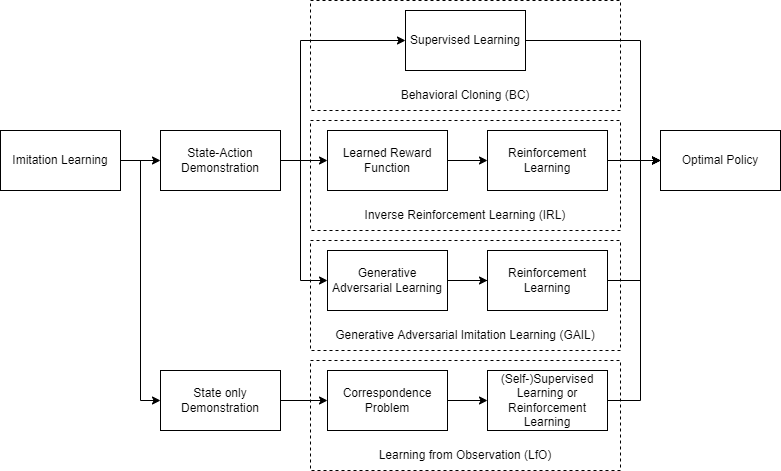
\includegraphics[width=0.9\textwidth]{Figures/images/il_taxonomy.png}
    \caption{Imitation Learning: Taxonomy and main components}
    \label{fig:il_methods}
\end{figure}


From Figure \ref{fig:il_methods}, it can be noted as IL and RL are strictly related, indeed, RL algorithms are used in
the training procedure of some methods, such as IRL, GAIL, and LfO. However, with respect to classic RL, IL allows to:
\begin{enumerate*}[label=\textbf{(\arabic*)}]
    \item bypass, or at least attenuate, the time-consuming exploration that would be required in a RL setting, 
    \item communicate, through demonstrations, a ``preference" for how a task should be performed.
    \item describe concepts that may be difficult to define formally or programmatically. \end{enumerate*}. As will be
explained in detail in Section \ref{sec:sota}, BC methods suffers of the \textit{compounding error} problem, since the
i.i.d. assumption that lays behind Supervised Learning is violated \cite{}. IRL was proposed to combine both the
data-efficiency of IL, to learn a reward function given the samples, and the exploration capability of RL, to attenuate
the \textit{compounding error} problem. However such methods have proved difficult to train. GAIL was proposed to reduce
the training complexity related to IRL, by framing the IRL problem as an Adversarial Learning problem, while the methods
improved both the performance and the efficiency of w.r.t. IRL methods, they showed poor performance when applied in
high-dimensional data, mainly due to the \textit{casual-confusion} problem \cite{}. LfO \cite{} was mainly proposed with
the aim to find a way to exploit state-only demonstrations, that are easy to obtain, and to collect. However, since
there is not any information about the true action,a way to measure the quality of prediction is needed. Moreover, the
\textit{correspondence problem}, i.e. how to map demonstration in human-space into the corresponding action in the robot
space, must be solved.     
\newline Despite all the open-challenges presented, IL was successfully applied for solving complex tasks, such as
driving a toy car \cite{codevilla2018end_to_end}, pick-and-place \cite{zhang2018deep}, and collaborative toolbox
assembly \cite{maeda2017probabilistic}, highlighting the high potential of such methods, which may justify an effort in
an attempt to resolve the gaps presented. A detailed description of the mentioned approaches will be given in
\textit{Section} \ref{sec:sota}, with an exhaustive comparison and description of the most recent and relevant methods.
%\noindent The need for a well-designed reward function, and the need for the system to interact with the environment
%during %the learning procedure, which is both time-consuming (e.g. in real-world experiments, at the end of each
%episode, the system %and the environment have to be put in the an initial state) and dangerous, are the main
%difficulties in using such approaches %in real-world application \cite{}. While the second drawback can be solved with
%the \textit{Offline RL}, 



\section{State-of-the-Art}
\label{sec:sota}
The chapter reviews the State-of-the-Art related to the \textit{Learning from Demonstration} problem. It will start with a general problem formulation (Section \ref{sec:problem_formulation}). Then it will briefly present the different methods used to collect data (Section \ref{sec:source_of_demonstration}). Next, the proposed methods will be explained and compared (Section \ref{sec:methods}). In the end, a summary will be presented, where a cross-approach comparison will be performed, and the current challenges will be emphasized (Section \ref{sec:summary}).
\subsection{Problem Definition}
\label{sec:problem_formulation}
Imitation Learning aims to obtain an agent that can replicate the behavior demonstrated by an expert agent. The behavior is described by a \textbf{policy}, where $\pi^{L}$ defines the learned policy, and $\pi^{E}$ defines the expert one. In the broadest possible definition, $\pi^{L}$ is obtained starting from a dataset $\mathcal{D}=\left \{ \left ( \boldsymbol{\tau}_{i}, \boldsymbol{c}_{i}\right ) \right \}_{i}^{N}$, where:
\begin{itemize}
    \item $\boldsymbol{\tau}_{i}$ is the $i^{th}$ demonstrated trajectory, which can be described as:
        \begin{itemize}
            \item A state-action sequence, i.e., $\boldsymbol{\tau}_{i} = [s_{0}, a_{0}, \dots, s_{T}, a_{T}]$, when it is assumed to have access to the ground-truth action performed by the expert.
            \item A state sequence, i.e., $\boldsymbol{\tau}_{i} = [s_{0}, \dots, s_{T}]$, when it is assumed to not have access to the ground-truth action.
        \end{itemize}    
    \item $\boldsymbol{c}_{i}$ is the \textit{context-vector}, it contains task-related information, e.g. the initial state of the system $s_{0}$, or the position of the target object.
\end{itemize}
The policy $\pi^{L}$ can be defined with respect to different abstraction levels \cite{fang2019survey,osa2018algorithmic}:   
\begin{enumerate*}[label=(\textbf{\alph*})]
    \item \textit{Symbolic Characterization}, the policy maps states, and context to a sequence of options, i.e., $\pi: s_{t}, \textbf{c} \rightarrow [o_1, \dots, o_T]$, where each option is a sequence of actions. With this representation, complex tasks can be decomposed into a sequence of simple movements. However, it is hard to achieve an accurate task segmentation and motion ordering.
    \item \textit{Trajectory Characterization}, the policy maps context to trajectory, i.e., $\pi: \mathbf{c} \rightarrow \boldsymbol{\tau}$. Because it allows the initial state to be mapped to a complete sequence of actions, this representation can be used to obtain the options in the Symbolic Representation. However, they need as many dynamic features as possible, that can be difficult to obtain.
    \item \textit{State-Action Characterization}, the policy maps states(-context) to actions, i.e., $\pi: s_{t}, \textbf{c} \rightarrow a_{t}$. This representation makes it possible to map the current state directly to the corresponding action. However, it is easy for errors to accumulate in long-term processes.
\end{enumerate*} 
\newline The agent, by means of its policy $\pi$, acts on a system, which is modeled as a \textit{Markov Decision Process} (MDP) \cite{kroemer2021review_robot_learning}. A MDP is defined as a tuple $(S,A,R,T,\gamma)$, where:
\begin{itemize}
    \item $S \subseteq \mathbb{R}^{n}$, is a set of states (e.g. joints position and/or image).
    \item $A \subseteq \mathbb{R}^{n}$, is a set of actions, (e.g. desired end-effector pose, desired joints torque).
    \item $R(s,a,s')$, is a \textit{reward function}, which expresses the immediate reward for executing action $a$ in state $s$, and transitioning to state $s'$.
    \item $T(s'|s,a)$ is a \textit{transition function}, which defines the probability to reach the state $s'$, after the execution of action $a$ in state $s$. This distribution, which describe the \textit{system dynamic}, that can be given a priori or learned (Model-Based methods), or do not taken into account (Model-Free methods).
    \item $\gamma \in [0,1]$, is a discount factor expressing the agent's preference for immediate over future rewards.
\end{itemize}
With respect to the given MDP definition, the reward function plays different roles based on the used approach. Indeed, in BC methods, the reward function is not implicitly used, but a surrogate loss-function is used instead. In IRL the reward function is learned, assuming that the expert acts (near-)optimal w.r.t. some unknown reward function. In GAIL and LfO, the rule played by the reward function is different based on the specific method, as will be explained in Section \ref{sec:methods}.
\subsection{Source of Demonstration [MAX 5]}
\label{sec:source_of_demonstration}
Regarding the way how the expert demonstrations can be obtained, according to \cite{fang2019survey}, two categories can be identified: \begin{enumerate*}[label=\textbf{(\alph*)}]
    \item Direct Demonstration. 
    \item Indirect Demonstration.
\end{enumerate*}
\input{Figures/direct_demonstration}
\paragraph{Direct Demonstration}  \mbox{} \\
\noindent It allows to obtain samples directly from the robot, either with kinesthetic teaching (Figure \ref{fig:kinesthetic}) or teleoperation teaching (Figure \ref{fig:teleoperation}). In kinesthetic teaching the human operator contacts and guides the robot, that collects data by itself, while in teleoperation teaching the human operator remotely guides the robot with joystick, tactile sensor, control panel, and wearable device. 
The former is characterized by the fact that there is no need to consider difference in kinematic between human and robot, as consequence, data has less noise. However, the robot must be passively controllable and require direct contact, introducing safety problems, and unintuitive demonstrations for robot with multiple degrees of freedom.
The latter is characterized by a higher safety, since there is no direct contact, and a wide application range.
A very popular example of teleoperation system is \textit{Roboturk} \cite{mandlekar2018roboturk}, it is a cloud-based teleoperation framework that enables the collection of high-scale demonstration dataset \cite{mandlekar2019scaling,mandlekar2022matters}, for both simulated and real-world robots, using a mobile-phone as controller (Figure \ref{fig:roboturk}). While this framework is interesting since it allows to collect data from a wide range of demonstrator with different demonstrations quality, it lacks of tactile information. When data are collected employing teleoperation, a way to collect contact information between the robot and the environment is represented by haptic interfaces \cite{cyberglove,touch}, which would allow the human operator to receive a force-feedback during the teleoperation task. However, the current literature has not yet focused on exploiting haptic information in the context of Learning from Demonstration, mainly due to the presence of open-challenges related to exploiting and best representing robot motion-related information, as will be explained in the following sections.
\input{Figures/roboturk}
\paragraph{Indirect Demonstration}  \mbox{} \\ 
It allows samples to be acquired in a way that is completely disconnected from the robotic platform. In this case the human motion is recorded by vision system (e.g. \cite{smith2019avid,sermanet2018time_contrastive}) or wearable device (e.g. \cite{liu2019_mirroring_without_overimitation}). In last years, the ability to extrapolate a policy starting from video of human performing a task has become a very important topic in the current literature \cite{fang2019survey,torabi2019recent_advances_lfo}. While Indirect Demonstration based on visual system allows to collect samples in the most intuitive and scalable way possible (potentially any video of performed task can be used), it lacks of tactile information, which can be obtained by using wearable devices such as gloves endowed with sensors able to measure the contact forces \cite{liu2017glove_force}. However, the correspondence problem must be solved, i.e. the system must be able to map motion captured in human space into the corresponding motion of the robot. In Section \ref{sec:lfo} the different ways how this problem has been solved in the context of visual demonstration will be explained in detail.

\newpage
\subsection{Methods}
\label{sec:methods}
\input{Chapters/1_background/sota_sections/bc}
\input{Chapters/1_background/sota_sections/irl}
\input{Chapters/1_background/sota_sections/gail}
\input{Chapters/1_background/sota_sections/lfo}
\newpage
\subsection{Summary}
\label{sec:summary}
This section summarizes all the approaches seen so far, trying to understand their pros and cons. Answering which approaches leads to better performance than the others is not trivial for several reasons ranging from the fact that, as mentioned above, methods are tested in different environments (e.g., some in simulation, others in the real world), on different tasks and using different robotic platforms. It can be said that, by analyzing the state of the art, the most studied approach is Behavioral Cloning. This approach, from a pure implementation point of view, is the simplest, as, in principle, it allows the execution of a purely offline training procedure. Unfortunately, some problems have to be handled, ranging from compounding-error to dataset creation. About the former, some solutions have been proposed, based on interactive learning algorithms, which reduce the covariate-shift phenomena, but introduce the need for active human supervision during the learning. During the past few years, there has been increasing interest in Meta-Learning algorithms, with the ultimate goal of achieving a system that can generalize across different tasks. However, as it turns out, the generalization problem is far from solved. 
Regarding approaches such as IRL, GAIL, and LfO. Compared to BC, methods such as IRL, GAIL, and LfO are more efficient regarding required demonstrations. However, they introduce RL algorithms into the optimization loop, which requires interaction with the environment, which can be risky and time-consuming. Moreover, despite their promising results, relatively few methods of these three approaches have actually been used in real-world vision-based manipulation tasks, effectively leaving unanswered the question of whether these methods can be used.


\chapter{Research Plan}
Based on the State of the Art, presented in Chapter \ref{sec:sota}, the following research-gaps can be identified ...., and the following questions can be made...

\chapter{Other Activities}
\label{chapter:other_activities}
\section{Attended Courses}
\subsection{Compulsary Courses}
The mandatory courses supported were:
\begin{itemize}
    \item \textit{Funding and Management of Research Project}. The course primarily emphasizes three aspects related to Research Projects: how to secure funding for a research project, how to craft a research proposal to obtain a grant, and how to effectively manage a project once the funding has been secured. First, the course introduced the European funding programs and their associated evaluation criteria. Particular attention was given to the Marie Skłodowska-Curie Actions (MSCA), specifically the Post-Doctoral Fellowship. Subsequently, the course covered project management methodologies, starting with an overview of project phases and the project life cycle, and concluding with concepts related to cost and risk management. Towards the conclusion of the course, we were tasked with composing a proposal for the MSCA Post-Doctoral Fellowship as the first part of the assignment, and a Project Management Plan and a First Year Report as the second part.
    \item \textit{Exploitation of Research Results}. The course is dedicated to presenting two strategies for leveraging research outcomes: the establishment of spin-off ventures and the creation of patents. In the initial segment, the regulations and methodologies employed to initiate a university spin-off have been presented. The subsequent section delves into the processes involved in crafting a patent. As a final activity, we were asked to prepare a proposal for a potential spin-off venture.
\end{itemize}
% \subsection{Additional Courses}
% I decided to add the following two exams to my path:
% \begin{itemize}
%     \item Mobile Robots for Critical Mission. The course, related to the Master Degree in Computer Engineering, aims to provide the architectural, methodological, and design elements for the realization of intelligent robots capable of moving autonomously in indoor environment. The course ended with the design, implementation, and validation of a software that allows a mobile robot platform to move autonomously, given the desired start and end points.
%     \item Ottimizzazione. The course aims to present the theoretical aspects related to both continuous and integer linear programming problems, combined with the respective solving algorithms.
% \end{itemize}
\section{Other Activities}
In conjunction with my primary research project centered on Robotic Learning from Demonstration, I was involved in a second research activity related to \textit{\textbf{Graph Representational Learning}} (GRL). GRL, which is a subfield of Machine Learning and Deep Learning, is dedicated to obtain valuable information from data structured in the form of graphs. This approach to data representation finds relevance in diverse domains, including but not limited to Recommendation Systems, Social Network Analysis, and Biological Networks, among others.

Under the supervision of Professor Pasquale Foggia and Professor Vincenzo Carletti, I directed my focus toward the topic of Anomaly Detection within the context of Internet-of-Things Device Networks. Our research aims to propose novel architectures and innovative learning paradigms to dynamically analyze such networks. The ultimate objective is to discern whether a subset of devices exhibits anomalous behaviors, an indicative sign that could potentially indicate the presence of cyber-attacks in progress. This pursuit not only enriches the field of Graph Representational Learning but also holds profound implications for the cybersecurity landscape.
\section{Mandatory requirements}

\subsection{International Conference as presenting author and Paper as corresponding author}
In the second year of our project, we did not produce any scientific publications for either conferences or journals. Nonetheless, because our initial findings presented intriguing insights, we are in the process of preparing a paper for the ``European Robotic Forum 2024" (ERF 2024), scheduled to take place in Rimini, Italy from March 13 to 15, 2024. The submission deadline for scientific materials is set for November 1, 2024.
In addition, we have intentions to expand and validate our current experiments, with the aim of creating another publication in reputable journals like ``IEEE Robotics and Automation Letters" (RA-L).

\subsection{Period Abroad}
I will spent the period abroad next year. We are currently assessing various opportunities with tutors who can enhance my skills, focusing on areas that complement what I've learned so far. These tutors will also provide valuable feedback on my research in AI-Enabled Robotics. Specifically, we are considering the tutorship with the following professors:
\begin{enumerate}
    \item \textit{Alberto Sanfeliu}, director of the Artificial Vision and Intelligent System Group (VIS) at the ``Universitat Polit`ecnica de Catalunya - Barcelona (Spain)" (UPC).  His research interests include intelligent robotics, human–robot interactions, computer vision, and pattern recognition.
    \item \textit{Francesc Serratosa}, full professor of Computer Science at the ``Universitat Rovira i Virgili - Tarragona (Spain)''. He appears in the list of the 2\% most influential researchers in the world, presented in ``Updated science-wide author databases of standardized citation indicators". He is active in research in the areas of Computer Vision, Machine Learning and Artificial Intelligence.
    \item \textit{Xiaoyi Jiang}, full professor of Computer Science at the University of Munster - Munster (Germany). His current research interests include 3D image analysis, and structural pattern recognition.
\end{enumerate}
\clearpage

\bibliography{bibliography.bib}
\addcontentsline{toc}{chapter}{Bibliography}

\clearpage

\end{document}